%========================================================================%
%               Copyright (C) 2016 All Rights Reserved.                  %
%             Author:BillHu<billhu@icloud.com>  Ver:<1.0>                %
%========================================================================%
%    The author grants permission, without fee and without a written     %
% license agreement, for use, reproduction, modification, and distribu-  %
% tion of this software and its documentation by educational, research,  %
% and non-profit entities for noncommercial purposes only.The above      %
% copyright notice and this paragraph MUST appear in all copies and      %
% modifications of the software and/or documentation.                    %
%========================================================================%
\documentclass{bjtu-bachelor-thesis}
\newcommand{\jnnote}[1]{\textcolor{red}{\small [#1]}}
\newcommand{\rynote}[1]{\textcolor{blue}{\small [#1]}}
\ctexset{chapter/break={}}
%========================================================================%
% 自定义内容
%========================================================================%
\ctitle{点阵图像和动画展示} %标题
\cmajor{计算机科学与技术}
\cauthor{张三} %作者
\cschool{计算机学院} %学院
\cid{21280000} %学号

%========================================================================%
% 前置部分
%========================================================================%

\begin{document}
\pagenumbering{roman}
\cover % 封面

\setcounter{page}{1}
\pagestyle{myfancy}

% 目录
\tableofcontents
\addcontentsline{toc}{part}{目\hspace{2em}录}%
\pagestyle{myfancy}
\clearpage
%\bibliographystyle{elsarticle-num}
%========================================================================%
% 主体部份
% 本示例文件以汇编实验报告模版为例,使用时可根据需求调整
%========================================================================%

\setcounter{page}{1}
\chapter{研究背景}

我们生活的世界正在不断被各种视听媒介塑造,图像、音乐、视频等媒体形式日益丰富,并在我们日常生活的各个领域广泛应用。然而,要理解这些媒体内容如何在微机上被存储、处理和呈现,我们需要深入研究底层系统的实现机制。

因此,我们计划设计并实现一个在微机上运行的系统,能够播放图像和音乐。这个系统将使用包括汇编语言和微机接口在内的技术,来处理和呈现这些媒体内容。这样的系统设计将使我们能够更深入地理解底层的系统实现,包括如何硬编码图像和音乐数据,以及如何通过微机接口将这些数据转换为用户可以感知的视觉和听觉体验。

具体来说,我们将以TPC-ZK综合开放式微机接口实验箱为实验平台,研究如何使用汇编语言来编码和处理图像和音乐数据,以及如何通过微机接口来实现这些处理。我们将探索如何精确地控制图像的显示和音乐的播放。

通过这个项目,我们希望能够提供一个能在微机上展示图像和音乐的实用系统,并能够提供一个深入理解底层系统实现的实践机会。这将对我们理解一个基本的计算机系统是如何运作以及掌握汇编语言有着重要的意义。

\chapter{研究内容}
% 点阵图像和动画展示,基于对图像的分析,将其图像以8x8的点阵来展示,并配有相应的音乐。将多张图片连续播放从而形成动画。

在本实验中,我们将通过TPC-ZK综合开放式微机接口实验箱中的特定元件(8255、8543、8259以及点阵显示模块),探索如何实现对应开关触发后,点阵显示出预定的动画内容并伴有相应的配乐。为此,我们设定了以下的设计目标:
    \begin{enumerate}
        \item 利用8259产生中断信号,以深化我们对中断信号生成机制的理解和实践。
        \item 通过8254产生定制的方波频率,为帧切换提供必要的频率服务。
        \item 应用8255进行数据传输。
        \item 熟悉点阵的编码方式, 讲对应帧硬编码至代码中。
    \end{enumerate}
\vspace{0.5cm}

\chapter{系统功能设计}

本设计共包含两个功能:
    \begin{enumerate}
        \item 通过操作实验箱上的开关,可以激活点阵以显示不同的图案,并同步产生对应的声音效果。当拨动两个或更多开关时,点阵将展示一个“X”图案。而在没有任何开关被操作的状态下,点阵将显示一个问号“?”图案,以提示等待开关输入。预计我们会设计5个开关,以支持显示5种不同的图像。
        \item 通过操作第6个开关,可以实现动画播放功能。利用定时器功能进行设定,我们将连续播放不同的图像,从而营造出动态的动画效果。
    \end{enumerate}
    
这种设计不仅实现了对点阵显示器的直观控制,还增添了音效和动画效果,使得用户交互体验更为丰富和有趣。
\vspace{0.5cm}

\chapter{系统实现}

    \begin{figure}[!htbp]
        \centering
        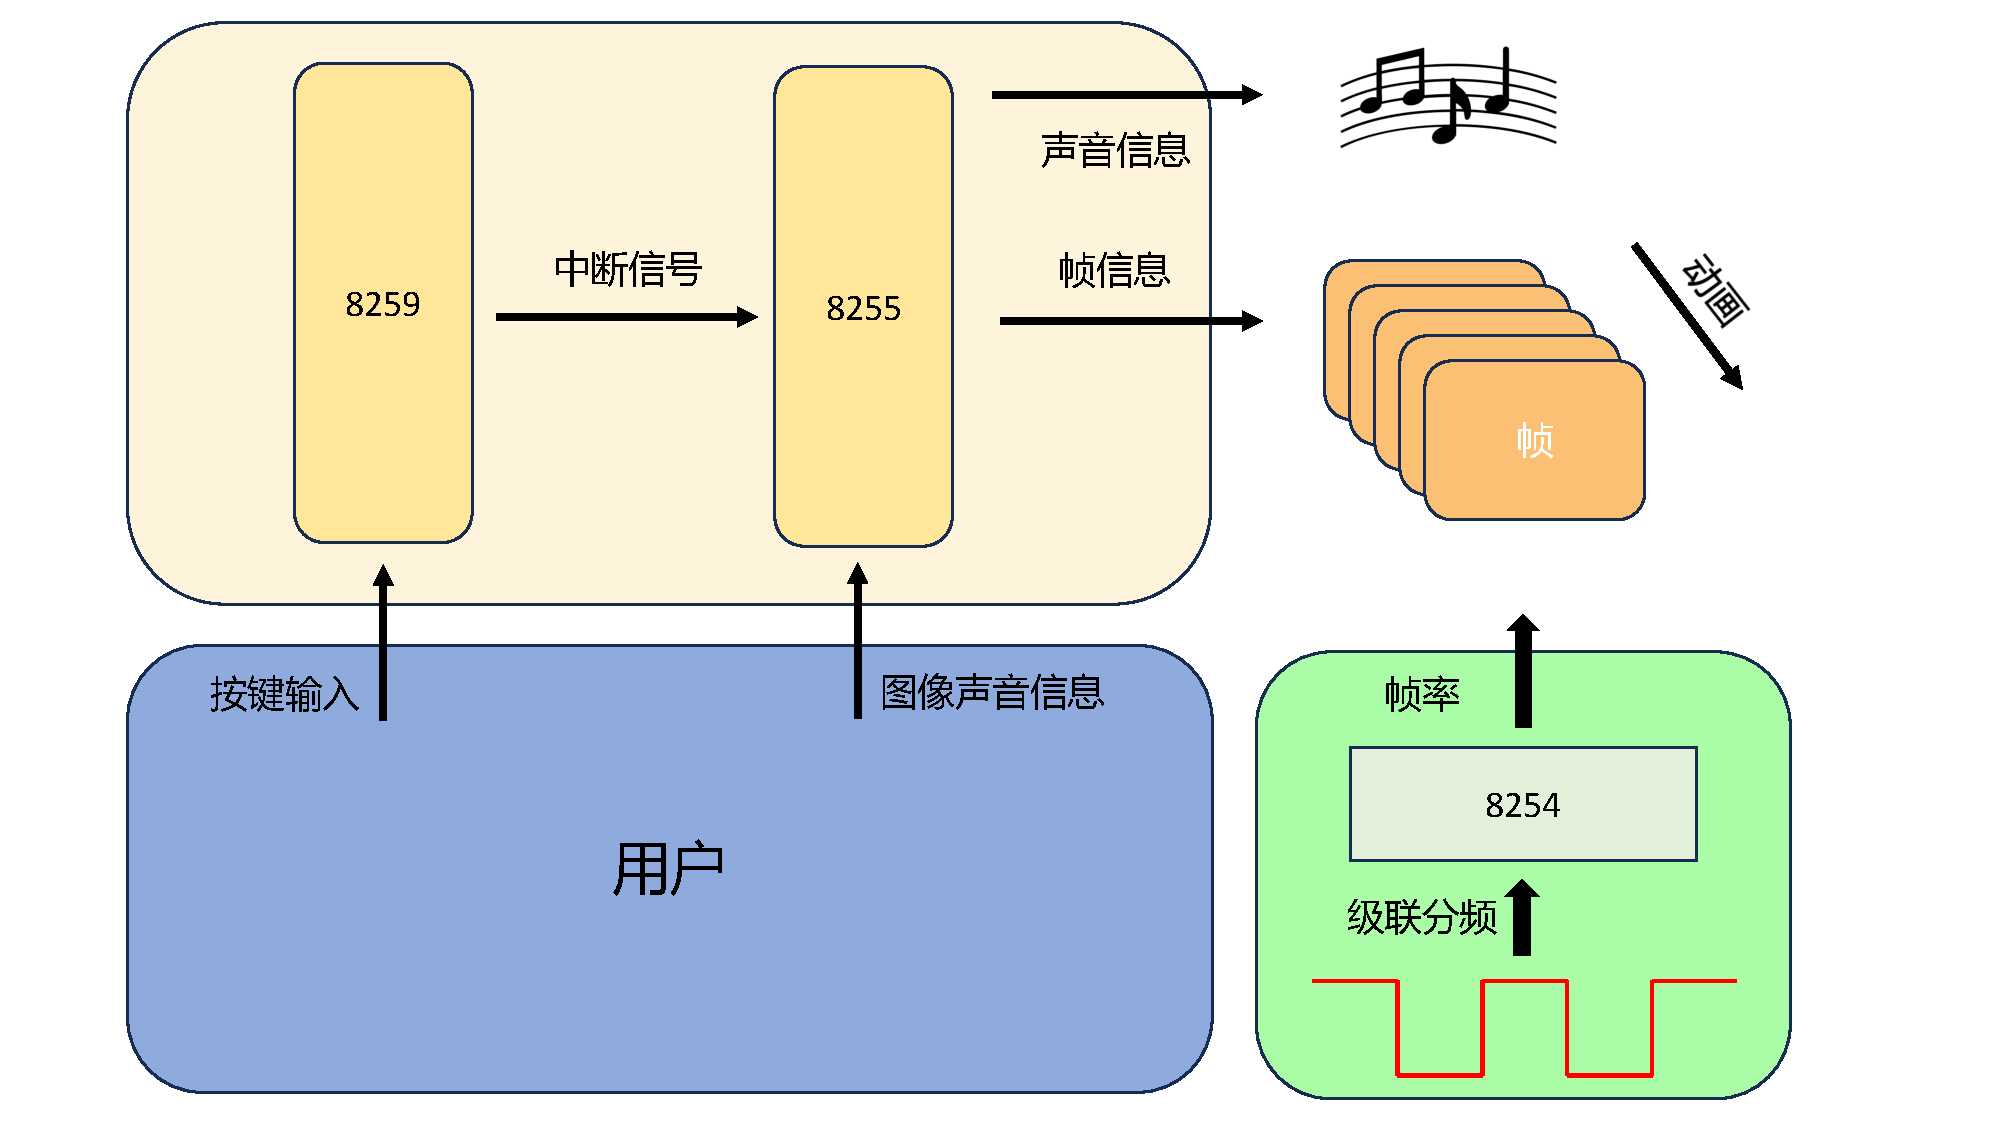
\includegraphics[width=1.0\textwidth]{pic/method.pdf}
        \caption{点阵图像和动画展示系统流程总览图}
        \label{fig:method}
    \end{figure}
    
图~\ref{fig:method}从总体展示了这个系统具体实现流程. 本设计包含两个核心功能,具体实现方式如下:
    \begin{enumerate}
        \item 通过8255和8259,我们能够实现不同拨码开关对应不同图像的显示。将拨码开关接入8259的一个输入端口,当检测到输入信号时,便会启动8255判断输入信号,之后通过8255的输出端口,驱动点阵显示相应的图案。如果当前开关被关闭,或者有其他拨码开关被激活,将终止当前中断,同时根据情况进入下一个中断,整个过程不断循环。
        \item 延时功能的实现将依赖8254,同样会用到8255和8259的协助。当开启动画播放的开关,8259会接收到输入信号,产生中断,通过8255判断输入的数据,如果为6则启动2号功能,让8254以产生特定频率的信号触发图片的切换,如此循环播放,直到接收到终止中断的信号。
    \end{enumerate}
    
这两个功能的设计,不仅能确保每个拨码开关都可以独立控制并显示特定的图像,同时也能够实现动画播放,使得整个系统的交互性和趣味性大大提升。


% 请注意以下使用方法
% 图片:
% \begin{figure}
%     \centering
%     \includegraphics{}
%     \caption{Caption}
%     \label{fig:my_label}
% \end{figure}

% 引用内部图片/表格
% \ref{}

% 引用外部文献
% \cite{}

% 列表
% 无序列表
% \begin{itemize}
%     \item 
% \end{itemize}
% 有序列表
% \begin{enumerate}
%     \item 
% \end{enumerate}

% \begin{table}[htbp]

%     \centering
%     \caption{国际单位制的基本单位}
%     \label{tbl:2-1}
%     \begin{tabularx}{0.8\textwidth}{*{3}{>{\centering\arraybackslash}X}}
%         \toprule
%         量的名称   & 单位名称     & 单位符号 \\ \midrule
%         长度       & 米           & m        \\
%         质量       & 千克(公斤)   & kg       \\
%         时间       & 秒           & s        \\
%         电流       & 安{[}培{]}   & A        \\
%         热力学温度 & 开{[}尔文{]} & K        \\
%         物质的量   & 摩{[}尔{]}   & mol      \\
%         发光强度   & 坎{[}德拉{]} & cd       \\ \bottomrule
%     \end{tabularx}
% \end{table}



\end{document}
